\chapter{High dimensional anomaly detection: HPC centers}


\section{Data}

The dataset is a time series with the following fields:
\begin{descriptionlist}
    \item[\texttt{timestamp}] with a $5$ minutes granularity.
    \item[HPC data] technical data related to the cluster.
    \item[\texttt{anomaly}] indicates if there is an anomaly.
\end{descriptionlist}

In practice, the cluster has three operational modes:
\begin{descriptionlist}
    \item[Normal] the frequency is proportional to the workload.
    \item[Power-saving] the frequency is always at the minimum.
    \item[Performance] the frequency is always at the maximum.
\end{descriptionlist}
For this dataset, both power-saving and performance are considered anomalies.


\subsection{High-dimensional data visualization}

\begin{description}
    \item[Individual plots]
        Plot individual columns.

    \item[Statistics]
        Show overall statistics (e.g., \texttt{pandas} \texttt{describe} method)

    \item[Heatmap]
        Heatmap with standardized data.

        \begin{figure}[H]
            \centering
            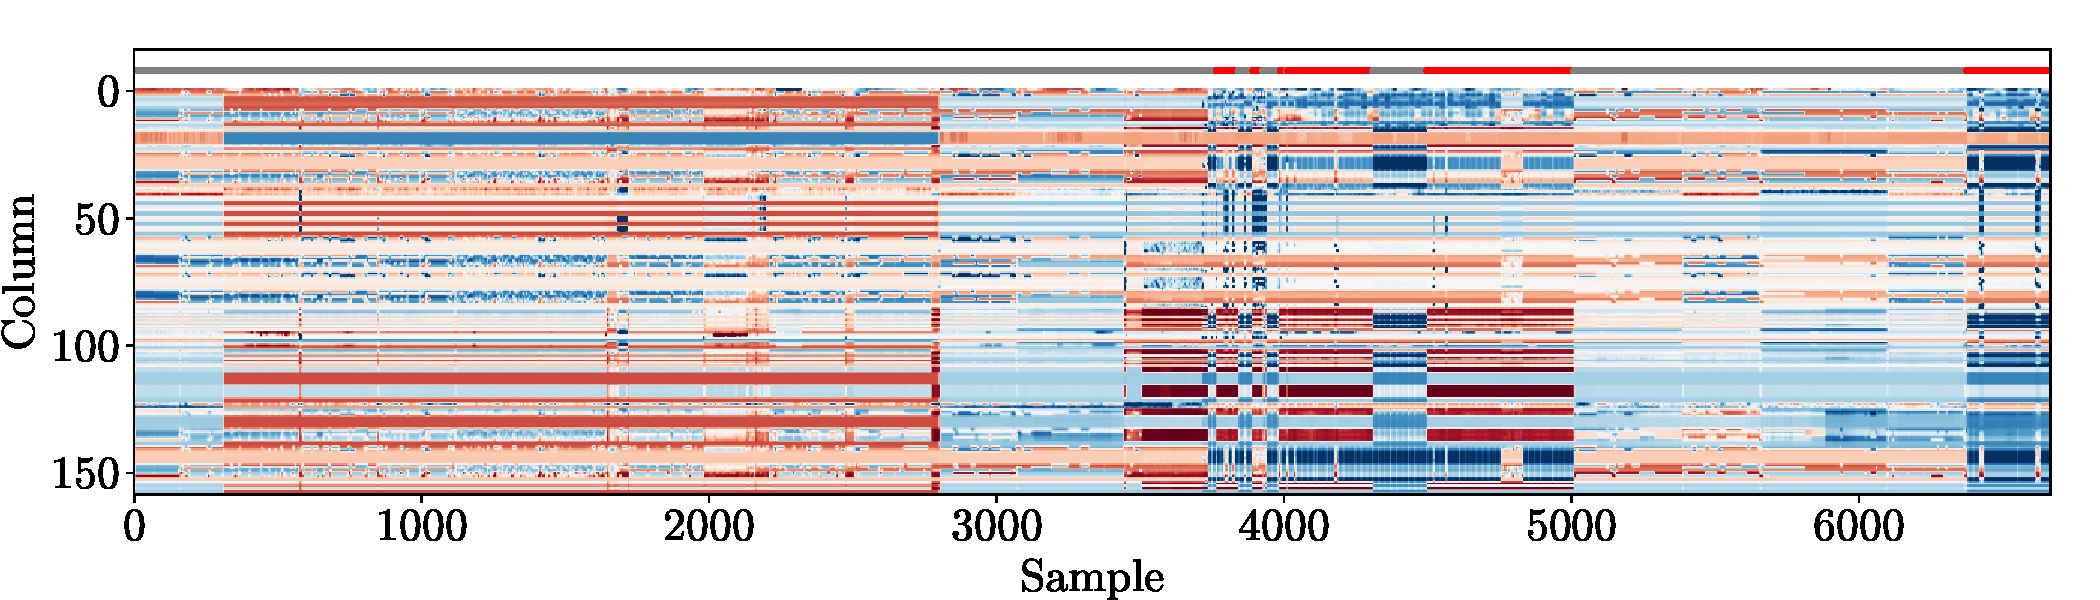
\includegraphics[width=0.9\linewidth]{./img/_ad_hpc_heatmap.pdf}
            \caption{
                \parbox[t]{0.75\linewidth}{Heatmap of the dataset. On the top line, gray points represent normal behavior while red points are anomalies. In the heatmap, white tiles represent the mean, red tiles represent values below average, and blue tiles represent values above average.}
            }
        \end{figure}
\end{description}



\section{Approaches}


\subsection{Multivariate KDE}

Given the train, validation, and test splits, the dataset is standardized using the training set alone. This avoids leaks from the test set.

The KDE model, bandwidth, and threshold are fitted as in \Cref{ch:ad_low}.

\begin{description}
    \item[Cost model]
        A simple cost model can be based on:
        \begin{itemize}
            \item False positives,
            \item False negatives,
            \item A time tolerance.
        \end{itemize}

    \item[Problems]
        KDE on this dataset has the following problems:
        \begin{itemize}
            \item It is highly subject to the curse of dimensionality and requires more data to be reliable.
            \begin{remark}
                KDE does not compress the input features and grows with the training set. In other words, it has low bias and high variance.
            \end{remark}

            \item As the dataset is used during inference, a large dataset is computationally expensive (with time complexity $O(mn)$, where $m$ is the number of dimensions and $n$ the number of samples).

            \item It only provides an alarm signal and not an explanation of the anomaly. In low-dimensionality, this is still acceptable, but with high-dimensional data it is harder to find an explanation.
        \end{itemize}
\end{description}


\subsection{Gaussian mixture model}

\begin{description}
    \item[Gaussian mixture model (GMM)] \marginnote{Gaussian mixture model (GMM)}
        Selection-based ensemble that estimates a distribution as a weighted sum of Gaussians. It is assumed that data can be generated by the following probabilistic model:
        \[ X_Z \]
        where:
        \begin{itemize}
            \item $X_k$ are random variables following a multivariate Gaussian distribution. The number of components is a hyperparameter that can be tuned to balance bias-variance.

            \item $Z$ is a random variable representing the index $k$ of the variable $X$ to use to generate data.
        \end{itemize}

        More specifically, the PDF of a GMM $g$ is defined as:
        \[ g(x, \mu, \Sigma, \tau) = \sum_{k=1}^{n} \tau_k f(x, \mu_k, \Sigma_k) \]
        where:
        \begin{itemize}
            \item $f$ is the PDF of a multivariate normal distribution.
            \item $\mu_k$ and $\Sigma_k$ are the mean and covariance matrix for the $k$-th component, respectively.
            \item $\tau_k$ is the weight for the $k$-th component and corresponds to $\prob{Z=k}$.
        \end{itemize}

        \begin{description}
            \item[Training]
                Likelihood maximization can be used to train a GMM to approximate another distribution:
                \[ \arg\max_{\mu, \Sigma, \tau} \mathbb{E}_{x \sim X} \left[ L(x, \mu, \Sigma, \tau) \right] \qquad \text{subject to } \sum_{k=1}^{n} \tau_k = 1 \]
                where the expectation can be approximated using the training set (i.e., empirical risk minimization):
                \[ \mathbb{E}_{x \sim X} \left[ L(x, \mu, \Sigma, \tau) \right] \approx \prod_{i=1}^{m} g(x_i, \mu, \Sigma, \tau) \]

                \begin{remark}
                    Empirical risk minimization can be solved in two ways:
                    \begin{itemize}
                        \item Use a single large sample (traditional approach).
                        \item Use many smaller samples (as in cross-validation).
                    \end{itemize}
                \end{remark}

                By putting the definitions together, we obtain the following problem:
                \[ \arg\max_{\mu, \Sigma, \tau} \prod_{i=1}^{m} \sum_{k=1}^{n} \tau_k f(x, \mu_k, \Sigma_k) \qquad \text{subject to } \sum_{k=1}^{n} \tau_k = 1 \]
                which:
                \begin{itemize}
                    \item Cannot be solved using gradient descent as it is an unconstrained method.
                    \item Cannot be solved using mixed-integer linear programming as the problem is non-linear.
                    \item Cannot be decomposed as the variables $\mu$, $\Sigma$, and $\tau$ appear in every term.
                \end{itemize}

                It is possible to simplify the formulation of the problem by introducing new variables:
                \begin{itemize}
                    \item A new latent random variable $Z_i$ is added for each example. $Z_i = k$ iff the $i$-th example is drawn from the $k$-th component. The PDF of the GMM can be reformulated to use $Z_i$ and without the summation as:
                    \[ \tilde{g}_i(x_i, z_i, \mu, \Sigma, \tau) = \tau_{z_i} f(x, \mu_k, \Sigma_k) \]
                    The expectation becomes:
                    \[ \mathbb{E}_{x \sim X, \{z_i\} \sim \{Z_i\}} \left[ L(x, z, \mu, \Sigma, \tau) \right] \approx \mathbb{E}_{\{z_i\} \sim \{Z_i\}} \left[ \prod_{i=1}^{m} \tilde{g}_i(x_i, z_i, \mu, \Sigma, \tau) \right] \]
                    Note that, as the distributions to sample $z_i$ are unknown, $Z_i$ cannot be approximated in the same way as $X$.

                    \item New variables $\tilde{\tau}_{i, k}$ are introduced to represent the distribution of the $Z_i$ variables. In other words, $\tilde{\tau}_{i, k}$ corresponds to $\prob{Z_i = k}$. This allows to approximate the expectation as:
                    \[ \mathbb{E}_{\hat{x} \sim X, \hat{z} \sim Z} \left[ L(\hat{x}, \hat{z}, \mu, \Sigma, \tau) \right] \approx \prod_{i=1}^{m} \prod_{k=1}^{n} \tilde{g}_i(x_i, z_i, \mu, \Sigma, \tau)^{\tilde{\tau}_{i, k}} \]
                    The intuitive idea is that, if $Z_i$ is sampled, $\tilde{\tau}_{i, k}$ of the samples would be the $k$-th component. Therefore, the corresponding density should be multiplied by itself for $\tilde{\tau}_{i, k}$ times.
                \end{itemize}

            Finally, the GMM training can be formulated as follows:
            \[ \arg\max_{\mu, \Sigma, \tau, \tilde{\tau}} \prod_{i=1}^{m} \prod_{k=1}^{n} \tilde{g}_i(x_i, z_i, \mu, \Sigma, \tau)^{\tilde{\tau}_{i, k}} \,\,\text{ s.t. } \sum_{k=1}^{n} \tau_k = 1, \forall i =1\dots m: \sum_{k=1}^{n} \tilde{\tau}_{i, k} = 1 \]
            which can be simplified by applying a logarithm and solved using expectation-maximization.
        \end{description}
\end{description}

\begin{remark}
    Differently from KDE, GMM allows making various types of prediction:
    \begin{itemize}
        \item Evaluate the (log) density of a sample.
        \item Generate a sample.
        \item Estimate the probability that a sample belongs to a component.
        \item Assign samples to a component (i.e., clustering).
            \begin{remark}
                GMM can be seen as a generalization of $k$-means.
            \end{remark}
    \end{itemize}
\end{remark}


\begin{remark}
    Differently from KDE, most of the computation is done at training time.
\end{remark}


\begin{description}
    \item[Number of components estimation] 
        The number of Gaussians to use in GMM can be determined through grid search and cross-validation.

        \begin{remark}
            Other method such as the elbow method can also be applied. Some variants of GMM are able to infer the number of components.
        \end{remark}

    \item[Threshold optimization]
        The threshold can be determined in the same way as in \Cref{sec:ad_taxi_kde_uni}.
\end{description}


\subsection{Autoencoder}

\begin{description}
    \item[Autoencoder] \marginnote{Autoencoder}
        Neural network trained to reconstruct its input. It is composed of two components:
        \begin{descriptionlist}
            \item[Encoder] $e(x, \theta_e)$ that maps an input $x$ into a latent vector $z$. 
            \item[Decoder] $d(z, \theta_d)$ that maps $z$ into a reconstruction of $x$.
        \end{descriptionlist}

        \begin{description}
            \item[Training]
                Training aims to minimize the reconstruction MSE:
                \[ \arg\min_{\theta_e, \theta_d} \left\Vert d\left( e(x_i, \theta_e), \theta_d \right) - x_i \right\Vert_2^2 \]

                To avoid trivial embeddings, the following can be done:
                \begin{itemize}
                    \item Use a small-dimensional latent space.
                    \item Use L1 regularization to prefer sparse encodings.
                \end{itemize}
        \end{description}


    \item[Autoencoder for anomaly detection]
        By evaluating the quality of the reconstruction, an autoencoder can be used for anomaly detection:
        \[ \Vert x - d(e(x, \theta_e), \theta_d) \Vert_2^2 \geq \varepsilon \]

        The advantages of this approach are the following:
        \begin{itemize}
            \item The size of the neural network does not scale with the training data.
            \item Neural networks have good performances in high-dimensional spaces.
            \item Inference is fast.
        \end{itemize}

        However, the task of reconstruction can be harder that density estimation.
\end{description}

\begin{remark}
    It is always a good idea to normalize the input of a neural network to have a more stable gradient descent. Moreover, with normalized data, common weight initialization techniques make the output approximately normalized too.
\end{remark}

\begin{remark}
    Counterintuitively, neural networks have a higher bias compared to traditional machine learning techniques for mainly two reasons:
    \begin{itemize}
        \item A change in a single parameter affects the whole network.
        \item Training using SGD inherently prevents overfitting. 
    \end{itemize}
\end{remark}


\begin{theorem}
    Under the following assumptions:
    \begin{itemize}
        \item Normally distributed noise (i.e., distance between prediction and ground truth),
        \item Independent noise among each output component (i.e., columns),
        \item Same variance (i.e., homoscedasticity) in the noise of each output component,
    \end{itemize}
    autoencoders are trained as density estimators.

    \begin{remark}
        When minimizing MSE, these assumptions hold.
    \end{remark}

    \begin{proof}
        When training an autoencoder $h$ using MSE on $m$ examples with $n$ features, the following problem is solved:
        \[ 
            \begin{split}
                \arg\min_{\theta} \Vert h(\vec{x}, \theta) - \vec{x} \Vert_2^2 
                    &= \arg\min_{\theta} \sum_{i=1}^{m} \sum_{j=1}^{n} (h_j(\vec{x}_i, \theta) - \vec{x}_{i,j})^2 \\
                    &= \arg\min_{\theta} \log\exp \left( \sum_{i=1}^{m} \sum_{j=1}^{n} (h_j(\vec{x}_i, \theta) - \vec{x}_{i,j})^2 \right) \\
                    &= \arg\min_{\theta} \log \prod_{i=1}^{m} \exp \left( \sum_{j=1}^{n} (h_j(\vec{x}_i, \theta) - \vec{x}_{i,j})^2 \right) \\
                    &= \arg\min_{\theta} \log \prod_{i=1}^{m} \exp \left( (h(\vec{x}_i, \theta) - \vec{x}_{i})^T \matr{I} (h(\vec{x}_i, \theta) - \vec{x}_{i}) \right)
            \end{split}
        \]
        The following adjustments can be done without altering the problem:
        \begin{itemize}
            \item Negate the argument of $\exp$ and solve a maximization problem,
            \item Multiply the argument of $\exp$ by $\frac{1}{2}\sigma$, for some constant $\sigma$,
            \item Multiply $\exp$ by $\frac{1}{\sqrt{2\pi}\sigma}$.
        \end{itemize}
        The problem becomes:
        \[ \arg\max_{\theta} \log \prod_{i=1}^{m} \frac{1}{\sqrt{2\pi}\sigma} \exp \left( -\frac{1}{2} (h(\vec{x}_i, \theta) - \vec{x}_{i})^T (\sigma\matr{I}) (h(\vec{x}_i, \theta) - \vec{x}_{i}) \right) \]
        which is the PDF of a multivariate normal distribution $f(\vec{x}_i, h(\vec{x}_i), \sigma\matr{I})$ with a diagonal covariance matrix. More specifically, this is a distribution:
        \begin{itemize}
            \item Centered on $h(\vec{x}_i)$,
            \item With independent normal components,
            \item With components with uniform variance.
        \end{itemize}

        Therefore, when using MSE as loss, training is a likelihood maximization problem.
    \end{proof}
\end{theorem}


\begin{description}
    \item[Threshold optimization]
        The threshold can be determined in the same way as in \Cref{sec:ad_taxi_kde_uni}.

    \item[Multiple signal analysis]
        With autoencoders, it is possible to compare the reconstruction error of single components. 

        \begin{remark}
            In most cases, reconstruction errors are often concentrated on a few features.

            \begin{figure}[H]
                \centering
                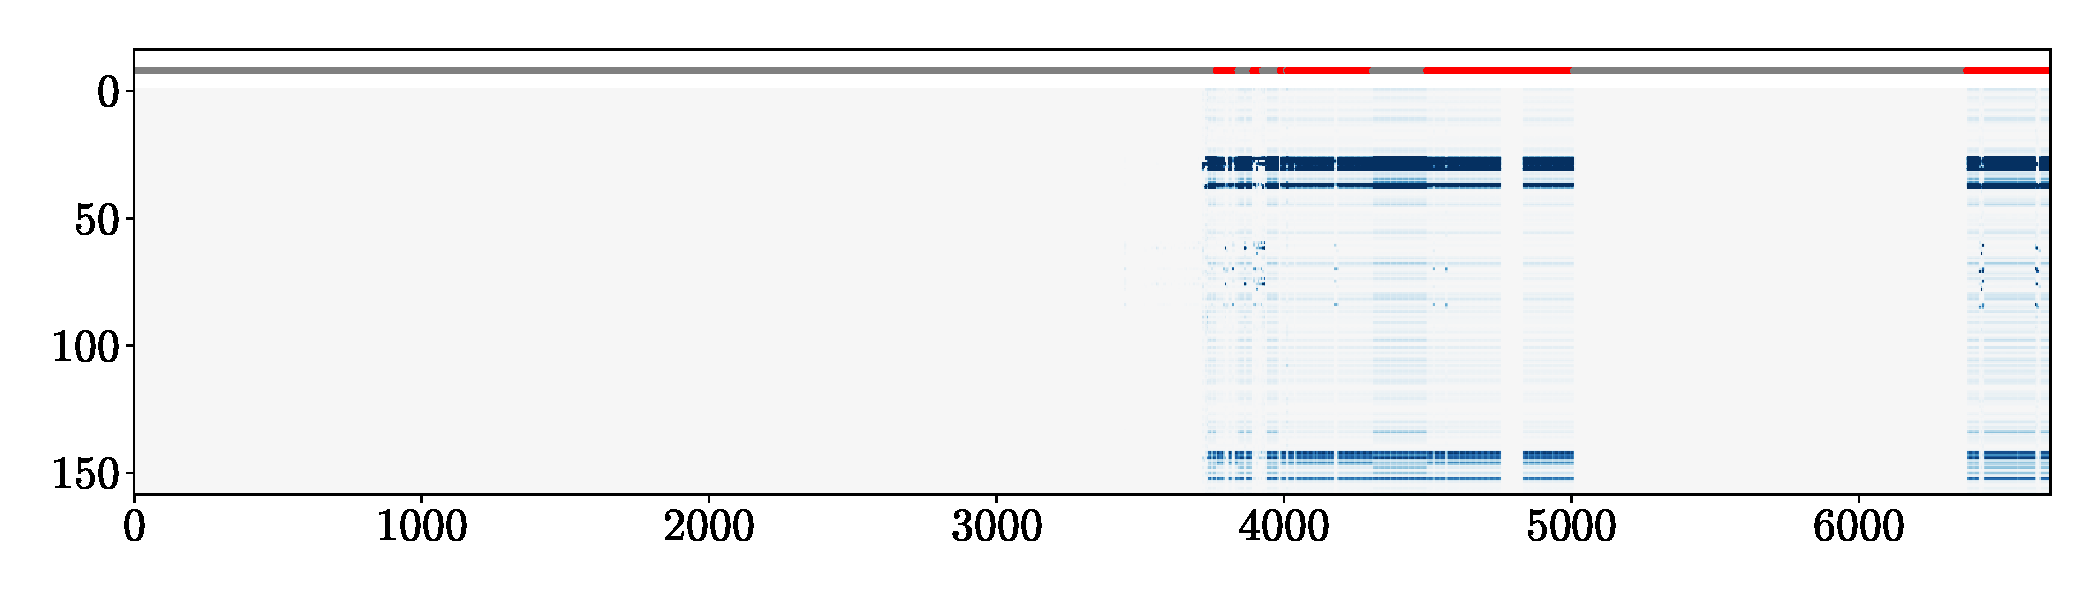
\includegraphics[width=0.8\linewidth]{./img/_ad_hpc_multi_signal.pdf}
                \caption{Reconstruction error of each feature}
            \end{figure}
        \end{remark}

        \begin{remark}
            It is possible to rank the feature with the highest reconstruction error to provide more insights.

            \begin{figure}[H]
                \centering
                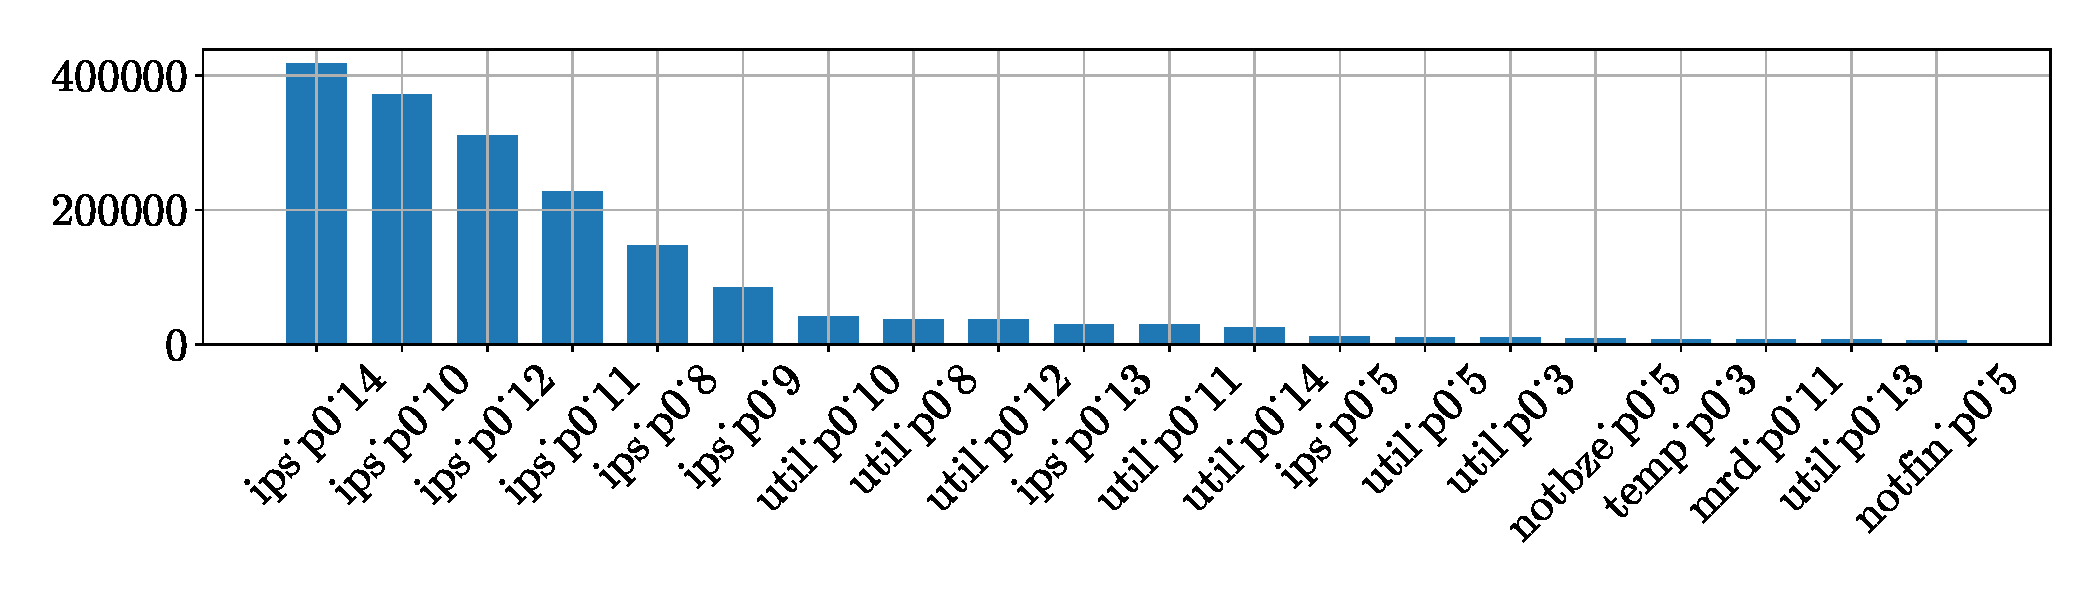
\includegraphics[width=0.8\linewidth]{./img/_ad_hpc_multi_signal_rank.pdf}
                \caption{Top-20 features with the largest error}
            \end{figure}
        \end{remark}
\end{description}


\begin{remark}
    In industrial use-cases, a usually well working approach consists of building an estimator for the sensors. More specifically, observed variables can be split into:
    \begin{itemize}
        \item Controlled variables $x_c$.
        \item Measured variables $x_s$.
    \end{itemize}
    During anomaly detection, controlled variables should not be used to determine anomalous behaviors. In addition, there is a causal relation between the two groups as measured variables are caused by the controlled variables ($x_c \rightarrow x_s$).

    A well working method is to use a regressor $f$ as a causal model, such that:
    \[ x_s \approx f(x_c; \theta) \]
\end{remark}